%%%%%%%%%%%%%%%%%%%%%%%%%%%%%%%%%%%%%%%%%%%%%%%%%%%%%%%%%%%%%%%%%%%%%%%
%%%                           System Description
%%%%%%%%%%%%%%%%%%%%%%%%%%%%%%%%%%%%%%%%%%%%%%%%%%%%%%%%%%%%%%%%%%%%%%




\chapter{Discussion}
We designed and implemented a role-playing game that puts the player as an attacker and shows different phishing techniques attackers can use.  Overall, we are pleased with the result of this first iteration of the game and its ability to convey educational materials.

\section{Insights}
We noticed a few common patterns during our study, and we believe additional training materials on these would help strengthen users against phishing attackers.

\subsection{Issues with subdomains}
Legitimate emails used in our survey used "info@mailer.netflix.com" as the sender, which is the email used by Netflix to send updates about user accounts. We noticed that participants marked these legitimate emails "Maybe phishing" or "phishing" although they were satisfied with other contents of the email.

We believe the confusion is mainly due to the following two reasons:

\begin{enumerate}
    \item Users are expecting the email to be from netflix.com. However, when users see "mailer" in the email, they get confused about the sender. We can see a similar example in ref{fig:lyft}. Lyft used "noreply@lyftmail.com" to send the email. This can easily confuse users, and attackers can potentially use similar patterns for other organizations to trick the victims.

    Notifying users with different domains used by organizations beforehand might help mitigate this issue.

    \item The issue mentioned in (1) also highlights another issue with current phishing training modules: subdomains. Although our game touches it briefly (and many games discussed in the literature review briefly cover it), we believe that dedicated training materials should be available to specifically cover the subdomain and train users on it.

\end{enumerate}

\begin{figure}
    \centering
    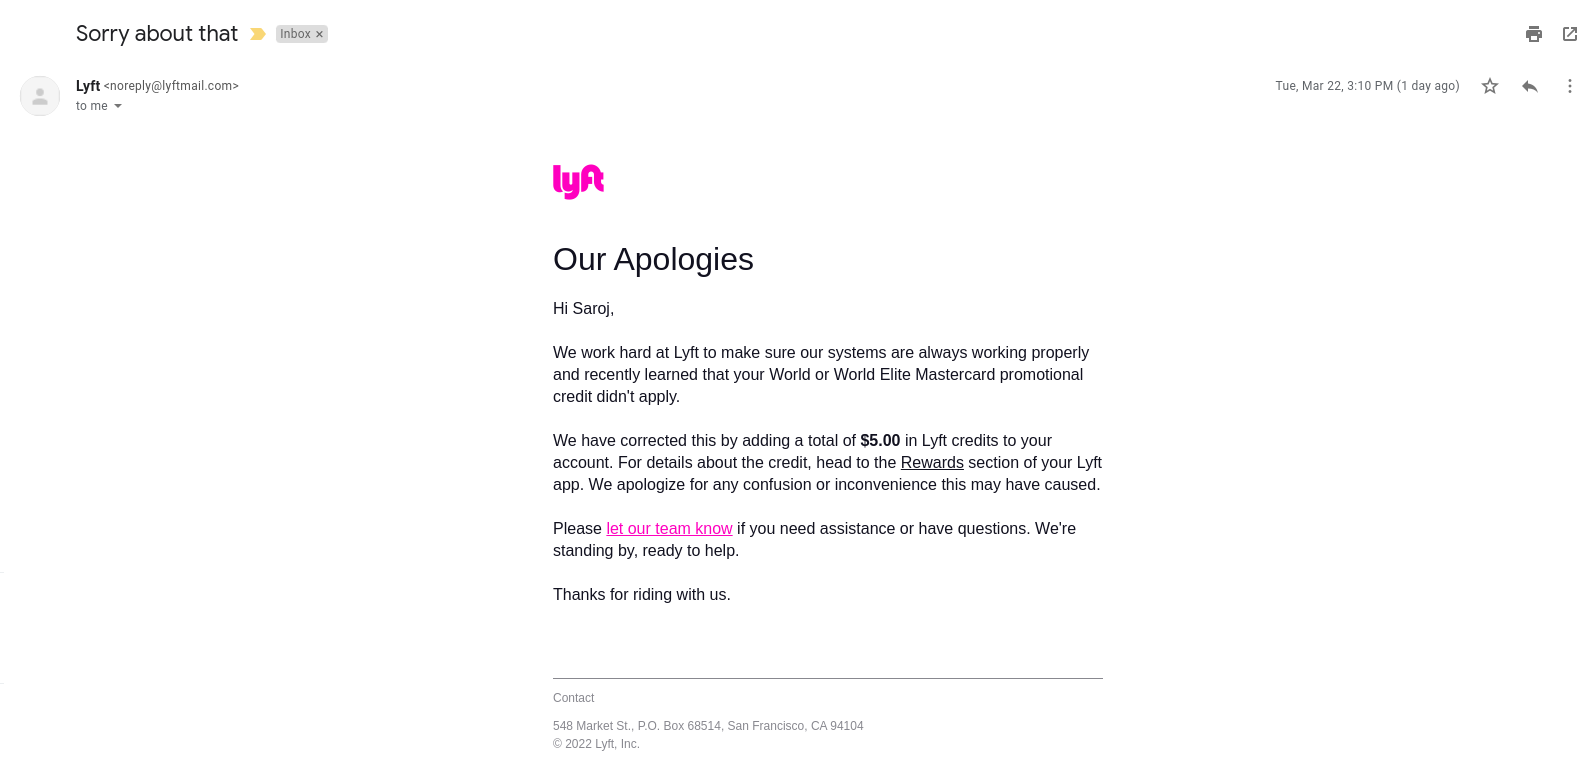
\includegraphics[width=\textwidth]{section4/lyft.png}
    \caption[An email sent by Lyft]{An email sent by Lyft. The sender of the email is \textit{noreply@lyftmail.com}}
    \label{fig:lyft}
\end{figure}

\subsection{Issues with email content}
Our pre-survey (and in some part post-survey) showed participants did not like when they got personal information (such as phone number and credit card number) in their email. We believe users would be more comfortable with such emails if they only notified the user of some change and gave the details in their platform.

\section{Limitations}
\section{Future Work}
\section{Conclusion}